\documentclass{article}

\usepackage{amsmath}
\usepackage{amsfonts}
\usepackage{amssymb}
\usepackage{booktabs}
\usepackage{geometry}
\usepackage{graphicx}
\usepackage{tcolorbox}
\usepackage{tikz}
\usepackage{xcolor}

\usetikzlibrary{arrows.meta, calc, patterns, positioning}

\geometry{a4paper, margin=1in}

\newcommand{\notesetup}[1]{
    \title{#1}
    \author{}
    \date{}
}

\newtcolorbox{keyidea}[1]{
    colback=blue!5,
    colframe=blue!45!black,
    title=#1
}

\newtcolorbox{pitfall}[1]{
    colback=red!4,
    colframe=red!55!black,
    title=#1
}


\usepackage{enumitem}
\usepackage{hyperref}
\usepackage{mathtools}
\usepackage{siunitx}

\hypersetup{colorlinks=true,linkcolor=blue,urlcolor=blue}
\sisetup{per-mode=symbol,detect-all}
\setlist[itemize]{nosep,leftmargin=*}
\setlist[enumerate]{nosep,leftmargin=*}

\newcommand{\dd}{\mathrm{d}}
\newcommand{\abs}[1]{\left|#1\right|}

\begin{document}

\notesetup{Simple Harmonic Motion}
\maketitle

\section{Hooke's Law}
For many students, the cleanest entry point to simple harmonic motion is the spring.

\textbf{Hooke's Law} states that, within the elastic limit of a spring, the spring force is proportional to the spring's extension or compression from its natural length:
\begin{equation}
    F_{\text{spring}} = -kx
\end{equation}
Here, $k$ is the spring constant and $x$ is the spring's deformation from its natural length.

When we study a mass oscillating about equilibrium, we usually redefine the coordinate so that displacement is measured from the equilibrium position. In that shifted coordinate, the restoring force still has the form $F=-kx$.

The negative sign matters. It tells us that the spring force always points in the direction opposite to the displacement.

\begin{center}
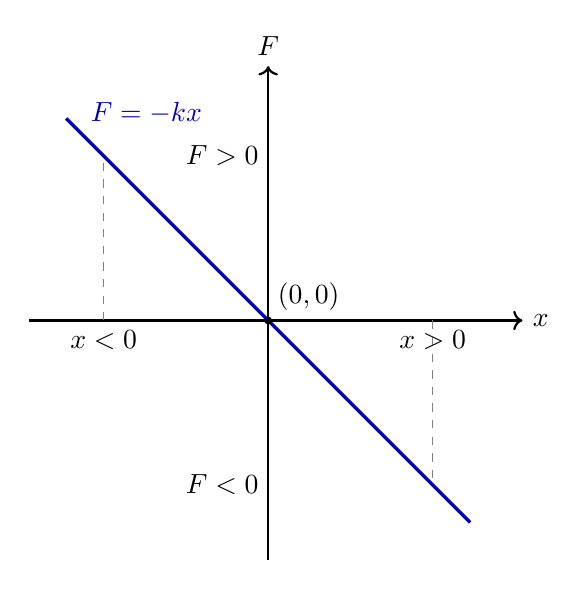
\begin{tikzpicture}[scale=0.95]
    \draw[->,thick] (-3.2,0) -- (3.4,0) node[right] {$x$};
    \draw[->,thick] (0,-3.2) -- (0,3.4) node[above] {$F$};
    \draw[blue!70!black,very thick] (-2.7,2.7) -- (2.7,-2.7);

    \draw[dashed,gray] (-2.2,0) -- (-2.2,2.2);
    \draw[dashed,gray] (2.2,0) -- (2.2,-2.2);

    \fill (0,0) circle (1.5pt) node[above right] {$(0,0)$};
    \node[below] at (-2.2,0) {$x<0$};
    \node[below] at (2.2,0) {$x>0$};
    \node[left] at (0,2.2) {$F>0$};
    \node[left] at (0,-2.2) {$F<0$};

    \node[blue!70!black,above right] at (-2.5,2.5) {$F=-kx$};
\end{tikzpicture}

\small A force-position graph for an ideal spring is a straight line through the origin with slope $-k$.
\end{center}

\begin{keyidea}{Physical Meaning of the Negative Sign}
If the mass is pulled to the right, the spring pulls it to the left. If the mass is pulled to the left, the spring pulls it to the right.
\end{keyidea}

\section{Restoring Force}
A \textbf{restoring force} is a force that acts to bring an object back toward equilibrium.

In a spring-mass system, the spring force is the restoring force. In other systems, the restoring force may be a net force or a component of a force rather than a single force by itself.

\textbf{Example:} In a simple pendulum, the restoring force is not the entire weight of the bob. It is the tangential component of gravity.

\section{What Makes a Motion SHM?}
Simple harmonic motion is a special kind of oscillation. A system undergoes SHM when the restoring force is proportional to displacement and opposite in direction:
\begin{equation}
    F_{\text{restoring}} \propto -x
\end{equation}
or, more specifically,
\begin{equation}
    F_{\text{net}} = -kx
\end{equation}

\begin{keyidea}{The Real Test for SHM}
Do not ask whether the object is moving back and forth. Ask whether the net restoring force is proportional to displacement from equilibrium.
\end{keyidea}

\section{Spring Oscillator}
For a frictionless horizontal spring-mass system, Hooke's Law gives
\begin{equation}
    F = -kx
\end{equation}
and Newton's second law gives
\begin{equation}
    F = ma
\end{equation}
so the acceleration must satisfy
\begin{equation}
    a = -\frac{k}{m}x
\end{equation}

This tells us that the acceleration is always directed toward equilibrium and that its magnitude grows with displacement.

\subsection*{Why the Motion Can Be Modeled with a Circle}
A useful way to understand SHM is to think of it as the projection of uniform circular motion onto one axis.

Imagine a point moving in a circle of radius $A$ with constant angular speed $\omega$. If we only track the $x$-coordinate of that point, its position is
\begin{equation}
    x = A\cos(\omega t)
\end{equation}

\begin{center}
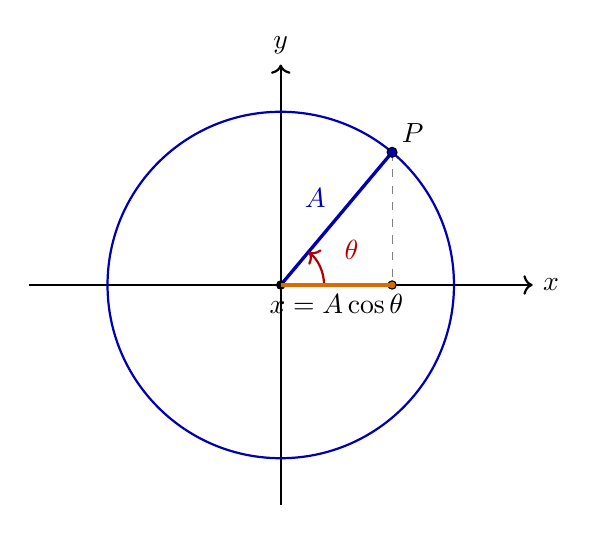
\begin{tikzpicture}[scale=1.0]
    \coordinate (O) at (0,0);
    \coordinate (P) at (50:2.2);
    \coordinate (Px) at (P |- O);

    \draw[->,thick] (-3.2,0) -- (3.2,0) node[right] {$x$};
    \draw[->,thick] (0,-2.8) -- (0,2.8) node[above] {$y$};
    \draw[blue!70!black,thick] (O) circle (2.2);
    \draw[very thick,blue!70!black] (O) -- (P) node[midway,above left] {$A$};
    \draw[dashed,gray] (P) -- (Px);
    \draw[fill=blue!70!black] (P) circle (1.8pt) node[above right] {$P$};
    \draw[fill=black] (O) circle (1.5pt);
    \draw[fill=orange!85!black] (Px) circle (1.5pt);

    \draw[thick,red!70!black,->] (0.55,0) arc[start angle=0,end angle=50,radius=0.55];
    \node[red!70!black] at (0.9,0.45) {$\theta$};

    \draw[very thick,orange!85!black] (O) -- (Px);
    \node[below] at ($(O)!0.5!(Px)$) {$x=A\cos\theta$};
\end{tikzpicture}

\small The horizontal projection of uniform circular motion behaves like simple harmonic motion.
\end{center}

This model immediately tells us two important facts:
\begin{itemize}
    \item The maximum displacement is $A$, so $A$ is the \textbf{amplitude}.
    \item The motion repeats whenever the angle increases by $2\pi$.
\end{itemize}

\subsection*{Deriving the Period}
In circular motion, one full cycle corresponds to an angle change of $2\pi$, so the period is
\begin{equation}
    T = \frac{2\pi}{\omega}
\end{equation}

Now connect this to the spring.

For the circular model, the acceleration along the $x$-direction is
\begin{equation}
    a_x = -\omega^2 x
\end{equation}

But for the spring-mass system, we already found
\begin{equation}
    a = -\frac{k}{m}x
\end{equation}

Since these describe the same motion,
\begin{equation}
    \omega^2 = \frac{k}{m}
\end{equation}
so
\begin{equation}
    \omega = \sqrt{\frac{k}{m}}
\end{equation}
and therefore
\begin{equation}
    T = \frac{2\pi}{\omega} = 2\pi\sqrt{\frac{m}{k}}
\end{equation}

\begin{keyidea}{What Determines the Period?}
For an ideal spring oscillator, the period depends only on $m$ and $k$.
\end{keyidea}

\subsection*{Deriving the Amplitude Idea}
From
\begin{equation}
    x = A\cos(\omega t)
\end{equation}
the largest possible value of $x$ is $A$ and the smallest possible value is $-A$. That is why amplitude is defined as the maximum displacement from equilibrium.

Amplitude is set by the \textbf{initial conditions}:
\begin{itemize}
    \item how far the object is initially displaced, or
    \item how large its initial speed is.
\end{itemize}

If the object is released from rest at maximum stretch, then that initial stretch is the amplitude.

\section{Amplitude and Period Are Not Related}
This point is extremely important.

For an ideal spring oscillator,
\begin{equation}
    T = 2\pi\sqrt{\frac{m}{k}}
\end{equation}
and this expression does \textbf{not} contain $A$.

That means:
\begin{itemize}
    \item increasing the amplitude changes the total energy,
    \item increasing the amplitude changes the maximum speed,
    \item but increasing the amplitude does \textbf{not} change the period.
\end{itemize}

\begin{keyidea}{High-Value Exam Fact}
In ideal SHM, amplitude and period are independent.
\end{keyidea}

\section{Position, Velocity, and Acceleration}
Even without full calculus, you should know the qualitative relationships:
\begin{itemize}
    \item At the endpoints $x=\pm A$, the speed is zero.
    \item At the endpoints, the acceleration magnitude is maximum.
    \item At equilibrium $x=0$, the acceleration is zero.
    \item At equilibrium, the speed magnitude is maximum.
    \item Acceleration always points toward equilibrium.
\end{itemize}

\begin{keyidea}{Endpoint vs Equilibrium}
Endpoint: $v=0$, $\abs{a}$ is maximum.\\
Equilibrium: $a=0$, $\abs{v}$ is maximum.
\end{keyidea}

\section{Small-Angle Pendulum}
A pendulum can also behave like SHM, but only for small angles.

\begin{center}
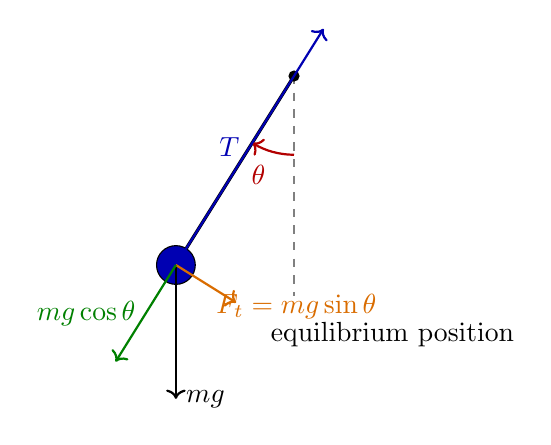
\begin{tikzpicture}[scale=1.0]
    \pgfmathsetmacro{\mglen}{1.7}
    \pgfmathsetmacro{\sinth}{0.53}
    \pgfmathsetmacro{\costh}{0.85}
    \coordinate (O) at (0,2.8);
    \coordinate (E) at (0,0);
    \coordinate (B) at (-1.5,0.4);
    \coordinate (Tdir) at ({0.85*\mglen*\sinth},{-0.53*\mglen*\sinth});
    \coordinate (Rdir) at ({-0.53*\mglen*\costh},{-0.85*\mglen*\costh});

    \draw[dashed,gray] (O) -- (E);
    \draw[very thick] (O) -- (B);
    \draw[fill=black] (O) circle (1.8pt);
    \draw[fill=blue!70!black] (B) circle (7pt);

    \draw[thick,red!70!black,->] (0,1.8) arc[start angle=-90,end angle=-122,radius=1.0];
    \node[red!70!black] at (-0.45,1.55) {$\theta$};

    \draw[->,thick] (B) -- ++(0,-\mglen) node[right] {$mg$};
    \draw[->,thick,blue!70!black] (B) -- ($(B)!1.25!(O)$) node[midway,left] {$T$};

    \draw[->,thick,orange!85!black] (B) -- ++(Tdir) node[midway,below right] {$F_t=mg\sin\theta$};
    \draw[->,thick,green!50!black] (B) -- ++(Rdir) node[midway,left] {$mg\cos\theta$};

    \node[below] at (1.25,-0.2) {equilibrium position};
\end{tikzpicture}

\small The restoring effect comes from the tangential component of gravity, not from the full weight $mg$.
\end{center}

Only the component of gravity along the tangent changes the bob's motion along the arc. The radial component is related to the tension and the bob's centripetal acceleration, but it is not the part that pulls the bob back toward equilibrium.

\begin{equation}
    F_t = -mg\sin\theta
\end{equation}

To turn this into the SHM form, we need one more step: for small angles measured in radians,
\begin{equation}
    \sin\theta \approx \theta
\end{equation}

\textbf{Why is this reasonable?} On a unit circle, the angle $\theta$ (in radians) is equal to the arc length, while $\sin\theta$ is the vertical coordinate. For very small angles, the arc, the chord, and the vertical rise are almost the same length, so $\sin\theta$ and $\theta$ are nearly equal.

\begin{keyidea}{Why Radians Matter}
The approximation $\sin\theta \approx \theta$ only works when $\theta$ is measured in radians. It is not true if $\theta$ is plugged in using degrees.
\end{keyidea}

So for a small-angle pendulum,
\begin{equation}
    F_t \approx -mg\theta
\end{equation}

Since the arc displacement is
\begin{equation}
    s = L\theta
\end{equation}
we can write
\begin{equation}
    F_t \approx -\frac{mg}{L}s
\end{equation}

This has exactly the same form as
\begin{equation}
    F = -kx
\end{equation}
which is why a small-angle pendulum behaves like SHM.

When the angle is small and measured in radians, this leads to the period formula
\begin{equation}
    T = 2\pi\sqrt{\frac{L}{g}}
\end{equation}
where $L$ is the pendulum length.

\textbf{Conditions for this formula:}
\begin{itemize}
    \item the angle must be small,
    \item the angle must be interpreted in radians,
    \item air resistance must be small,
    \item the bob is treated as a particle and the string as light.
\end{itemize}

\begin{keyidea}{Spring vs Pendulum}
For a spring oscillator, $T$ depends on $m$ and $k$. For a small-angle pendulum, $T$ depends on $L$ and $g$.
\end{keyidea}

\section{Energy in SHM}
For a spring oscillator, the elastic potential energy is
\begin{equation}
    U = \frac{1}{2}kx^2
\end{equation}

The total mechanical energy is
\begin{equation}
    E = K + U = \frac{1}{2}mv^2 + \frac{1}{2}kx^2
\end{equation}

If there is no energy loss, then the total mechanical energy stays constant.

At the endpoints, $v=0$, so all the energy is elastic potential energy:
\begin{equation}
    E = \frac{1}{2}kA^2
\end{equation}

Therefore, at any point in the motion,
\begin{equation}
    \frac{1}{2}mv^2 + \frac{1}{2}kx^2 = \frac{1}{2}kA^2
\end{equation}

From this, we can solve for speed:
\begin{equation}
    v = \pm \sqrt{\frac{k}{m}(A^2-x^2)}
    = \pm \omega\sqrt{A^2-x^2}
\end{equation}

\begin{keyidea}{Energy Shortcut}
Many SHM questions are easier with energy than with force analysis.
\end{keyidea}

\section{Example Problem 1}
\textbf{Problem:} A \SI{0.40}{kg} mass is attached to a spring of constant \SI{160}{N/m}. Find the period of the oscillation.

\textbf{Solution:}
\begin{equation}
    T = 2\pi\sqrt{\frac{m}{k}}
      = 2\pi\sqrt{\frac{0.40}{160}}
      = 2\pi\sqrt{0.0025}
      = 2\pi(0.05)
      \approx \SI{0.314}{s}
\end{equation}

\section{Example Problem 2}
\textbf{Problem:} A spring oscillator has $m=\SI{0.50}{kg}$, $k=\SI{200}{N/m}$, and amplitude $A=\SI{0.10}{m}$. Find the speed when the mass is at $x=\SI{0.06}{m}$.

\textbf{Solution:}
\begin{equation}
    \frac{1}{2}mv^2 + \frac{1}{2}kx^2 = \frac{1}{2}kA^2
\end{equation}
\begin{equation}
    \frac{1}{2}(0.50)v^2 + \frac{1}{2}(200)(0.06)^2 = \frac{1}{2}(200)(0.10)^2
\end{equation}
\begin{equation}
    0.25v^2 + 0.36 = 1.00
\end{equation}
\begin{equation}
    0.25v^2 = 0.64
    \qquad \Rightarrow \qquad
    v^2 = 2.56
\end{equation}
\begin{equation}
    v = \SI{1.6}{m/s}
\end{equation}

\section{Common Pitfalls}
\begin{pitfall}{Watch Out}
\begin{itemize}
    \item Do not measure displacement from an arbitrary origin. Measure it from equilibrium.
    \item Do not forget that the restoring force points opposite to displacement.
    \item Do not assume that larger amplitude means larger period.
    \item Do not use the pendulum period formula unless the angle is small.
    \item Do not confuse maximum displacement with maximum speed.
\end{itemize}
\end{pitfall}

\end{document}
